\input format.tex

\usepackage{graphicx}
\graphicspath{{cores/}}

\usepackage{environ}
\usepackage{colortbl,array,booktabs}
\usepackage{tabularx}

\colorlet{TablaBordeSuperior}{topcolor}
\colorlet{TablaBordeInferior}{topcolor}
\colorlet{TablaCentroSuperior}{blue!1}
\colorlet{TablaCentroInferior}{blue!20}
\colorlet{FuenteCabeceraTabla}{white}

\newcolumntype{M}[1]{>{\centering\arraybackslash}m{#1}}
%\newcommand{\tabularxcolumn}[1]{>\arraybackslash}m{#1}}

\tcbset{rtab/.style={
freelance,
frame code={
 \path[top color=topcolor,bottom color=topcolor]
   ([yshift=-#1*(\baselineskip+2pt)]interior.north west) --
   ([yshift=-#1*(\baselineskip+2pt)]interior.north east) {[sharp corners]--
    ([yshift=3pt]interior.north east) --
    ([yshift=3pt]interior.north west)} -- cycle;

  },
interior code={},
 }
}

\newcommand\fuentecabecera[1]{\textcolor{black}{\textbf{#1}}}

\begin{document}

\vspace*{5mm}
%% 各章节
\setlength{\arrayrulewidth}{.2pt}
\fontsize{9.3pt}{11pt}\selectfont
\color{gray2}

\begin{center}
{\noindent\bf\sanhao 一、检测结果总评}
\end{center}

\vspace*{3mm}

%\noindent{\bf{检测结果总体评价}}
\begin{CRaside}[.45]{\bf\xiaowuhao{体重:51.0kg \quad BMI:19.92 \quad 正常}}
\\
减肥难易程度\\\\

\includegraphics{difficulty-l4.pdf}
\asidebreak %
\\
减肥所需预估时间\\\\

\includegraphics{regulatetime-l3.pdf}
\end{CRaside}

\vspace*{4mm}

\begin{tctabularx}{tabularx={m{4cm}<{\centering}m{6.6cm}<{\centering}m{4cm}<{\centering}}}
&&
\\[-6pt]
\cellcolor{topcolor} \raisebox{2.614pt}{\color{gray0}\bf 检测项目} &
\cellcolor{topcolor} \raisebox{2.614pt}{\color{gray0}\bf 健康状态提示} &
\cellcolor{topcolor} \raisebox{2.614pt}{\color{gray0}\bf 检测结果评价}
\end{tctabularx}

\vspace*{-4.25mm}
\fontsize{8pt}{10pt}\selectfont
\arrayrulecolor{gray2}
\begin{longtable}{m{4cm}<{\centering}m{6.6cm}<{\centering}m{0cm}@{}m{4cm}<{\centering}}
\hline
\parbox[c]{\hsize}{\vskip7pt {\lantxh 微生态平衡能力} \vskip7pt} & \parbox[c]{\hsize}{\vskip7pt\centerline{\raisebox{-1.5ex}{
\includegraphics[width=6cm,height=0.55cm]{bar01.pdf}}}\vskip7pt}  &
\hspace*{-5.08cm}\raisebox{-0.75ex}{
\includegraphics{cry.pdf}}
 & \begin{minipage}{4cm}\begin{center}{{\lantxh 较差} }\end{center} \end{minipage} \\
\hline
\parbox[c]{\hsize}{\vskip7pt {\lantxh 胖菌} \vskip7pt} & \parbox[c]{\hsize}{\vskip7pt\centerline{\raisebox{-1.5ex}{
\includegraphics[width=6cm,height=0.55cm]{bar02.pdf}}}\vskip7pt}  &
\hspace*{-5.08cm}\raisebox{-0.75ex}{
\includegraphics{smile.pdf}}
 & \begin{minipage}{4cm}\begin{center}{{\lantxh 偏低} }\end{center} \end{minipage} \\
\hline
\parbox[c]{\hsize}{\vskip7pt {\lantxh 瘦菌} \vskip7pt} & \parbox[c]{\hsize}{\vskip7pt\centerline{\raisebox{-1.5ex}{
\includegraphics[width=6cm,height=0.55cm]{bar01.pdf}}}\vskip7pt}  &
\hspace*{-5.08cm}\raisebox{-0.75ex}{
\includegraphics{cry.pdf}}
 & \begin{minipage}{4cm}\begin{center}{{\lantxh 偏低} }\end{center} \end{minipage} \\
\hline
\end{longtable}

\begin{spacing}{1.5}
\indent
建议您通过调节肠道菌群,提高微生态平衡能力;增加瘦菌含量,改变易胖菌群体质,科学减肥,轻松又健康。(根据本检测结果将量身定制具体的减重方案,详情请咨询我司的专业团队)
\end{spacing}

\vspace*{10mm}

\noindent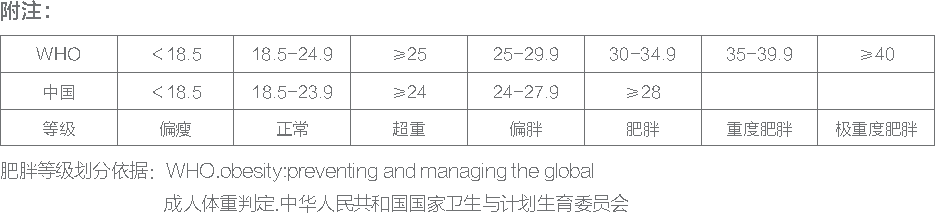
\includegraphics[width=\linewidth]{BMI_info.pdf}

\end{document}
